\chapter{Órbitas gravitatorias}

\section{Órbitas posibles el la interacción gravitatoria}
\begin{miparrafo}
	En física, una órbita es la trayectoria que describe un objeto físico alrededor de otro mientras está bajo la influencia de una fuerza central, como la fuerza gravitatoria.

El estudio de las órbitas se inicia con la aportación matemática de Johannes Kepler, quien fue el que formuló los resultados en sus tres leyes del movimiento planetario. La primera, propuso que las órbitas de los planetas en el sistema solar son elípticas y no circulares o epiciclos, como se pensaba antes, y que el Sol no se encontraba en el centro de sus órbitas sino en uno de sus focos. La segunda, que la velocidad orbital de cada planeta no es constante, como también se creía, sino que la velocidad del planeta depende de la distancia entre el planeta y el Sol. Y la tercera, Kepler encontró una relación universal entre las propiedades orbitales de todos los planetas orbitando alrededor del Sol. Para cada planeta, la distancia entre el planeta y el Sol al cubo, medida en unidades astronómicas, es igual al periodo del planeta al cuadrado, medido en años terrestres.

Isaac Newton demostró que las leyes de Johannes Kepler se derivaban de su teoría de la gravedad y que, en general, las órbitas de los cuerpos que respondían a la fuerza gravitatoria eran secciones cónicas. Isaac Newton demostró que un par de cuerpos siguen órbitas de dimensiones que son inversamente proporcionales a sus masas sobre su centro de masas común. Cuando un cuerpo es mucho más masivo que el otro, se hace la convención de tomar el centro de masas como el centro del cuerpo con mayor masa.
\end{miparrafo}

Segunda ley de Newton aplicada a la interacción gravitatoria entre dos cuerpos:

$\displaystyle \mu \dv[2]{\vec r}{t}=-G \dfrac{M+m}{r^2} \ \vec u_r ;\quad \mu=\dfrac{Mm}{M+m} \quad \to \ \quad \dv[2]{\vec r}{t}=-G \dfrac{Mm}{r^2} \ \vec u_r$

En polares: 

$\displaystyle \dv[2]{\vec r}{t}=\left[ \dv[2]{r}{t}-r\left( \dv{\theta}{t}\right)^2  \right]\ \vec u_r + \left[ 2r \dv{r}{t} \dv{\theta}{t}+r^2\dv[2]{\theta}{t}  \right] \ \vec u_\theta = - G \dfrac{M+m}{r^2} \vec u_r$

Como la fuerza gravitatoria que actúa es radial, solo tiene componente en la dirección de $\vec u_r$, la componente en la dirección de $\vec u_\theta$ ha de ser cero.

$\displaystyle 2r \dv{r}{t} \dv{\theta}{t}+r^2\dv[2]{\theta}{t}=0  \to  \dv{t} \left( r^2 \dv{\theta}{t} \right) =0  \to  r^2 \dv{\theta}{t}=cte(*)=\dfrac{L_{CM}}{\mu}$ 
(*)\footnote{Visto en ecuación \ref{ele-mu}}

Y nos queda que:  $\ \displaystyle  \dv[2]{r}{t}-r\left( \dv{\theta}{t}\right)^2=- G \dfrac{M+m}{r^2}$, 

despejando $\dv {\theta}{t}$ de (*) y sustituyendo:
$\ \displaystyle \dv[2]{r}{t} -\dfrac{L^2_{CM}}{\mu^2r^3}=-G\dfrac{M+m}{r^2}$ (**)

Notación: vamos a llamar $\ \displaystyle \dot{r}=\dv{r}{t}$, con lo cual establecemos un cambio de variable:

$\displaystyle \dv[2]{r}{t}=
\dv{t} \left( \dv{r}{t} \right)=\dv{t} \dot{r} =
\dv{r} \dv{r}{t} \dot{r}=
\dv{r}{t} \dv{\dot{r}}{r}=
\dot{r}\dv{\dot{r}}{r}$

Ya podemos integrar en (**): $\ \ \displaystyle \dot{r} \ \dv{\dot{r}}{r}=\dfrac{L^2_{CM}}{\mu^2} \ r^{-3}-G(M+m) \ r^{-2}$

$\displaystyle \int \dot{r}\  \dd \dot{r}=\int \left[ \dfrac{L^2_{CM}}{\mu^2} \ r^{-3}-G(M+m) \ r^{-2} \right] \ \dd r$

Como no hemos fijado los límites de integración, aparecerá una cte.

$\displaystyle \dfrac {{\dot{r}}^2}{2}=-\dfrac{L^2_{CM}}{2\mu^2} \ r^{-2} + G(M+m)\ r^{-1}+cte \to {\dot{r}}^2 =-\dfrac{L^2_{CM}}{\mu r^2}  + \dfrac{2G(M+m)}{r}  +k'$

\begin{equation}
	\label{r-punto-cuadrado}
	{\dot{r}}^2 \ =\ -\dfrac{L^2_{CM}}{\mu^2 \ r^2}  \ +\  G(M+m) \left[ \dfrac 2 r +k \right]
\end{equation}

Vamos a calcular la velocidad, en módulo, de un planeta alrededor de otro en cada instante, para ello, recordando la forma del vector velocidad en polares (ec. \ref{veloc-polares}):

$\displaystyle \vec v= \vec u_r \ \dv{r}{t}+ \vec u_\theta \ r \ \dv{\theta}{t}=\vec u_r \ \dot{r}+ \vec u_\theta \ r\  \dot{\theta} \ \to \ v^2={\dot{r}}^2+{(r \ \dot{\theta})}^2; \quad \dot{\theta}=\dfrac{L_{CM}}{\mu\ r^2}$

$\displaystyle v^2=- \bcancel{\dfrac{L^2_{CM}}{\mu^2\ r^2}} \ + \ G(M+m)\left( \dfrac 2 r  + k \right)+ \bcancel{ \cancel{r^2} \dfrac{L^2_{CM}}{\mu^2 \cancelto{2}{r^4}} }$

\begin{equation}
\label{v-cuadrado}
v^2 \ = \ G\ (M+m) \ \left( \dfrac 2 r + k \right)	
\end{equation}

Seguimos con la ecuación (\ref{r-punto-cuadrado}) y hacemos, de nuevo, otro cambio de variable, esta vez con $\dot{\theta}$:
$\quad \displaystyle \dot{r}=\dv{r}{t}=\dv{r}{\theta} \ \dv{\theta}{t}=\dv{r}{\theta}\  \dot{\theta}$

$\textcolor{gris}{\dot{\theta}=\dfrac{L_{CM}}{\mu\ r^2} \ \to \ \dfrac{L^2_{CM}}{\mu^2r^2}=\dfrac{(\dot{\theta} \mu r^2)^2}{\mu^2 r^2}=r^2 {\dot{\theta}}^2  ; \quad \quad {\dot{\theta}}^2= \dfrac{L^2_{CM}}{\mu^2r^4} }$



$\displaystyle \left( \dv{r}{\theta} \right)^2 \ {\dot{\theta}}^2 \ = \ -r^2 \  {\dot{\theta}}^2 \ + \ G\ (M+m)\ \left( \dfrac 2 r + k \right) $

$\displaystyle \left( \dv{r}{\theta} \right)^2 \ = \ 
-r^2 + \dfrac{ G (M+m) \left( \dfrac 2 r + k \right) }{ \dfrac{L^2_{CM}}{\mu^2\ r^4} } \ = \ -r^2 \ + \  \dfrac{  \mu^2r^4G(M+m)}{L^2_{CM}} \left( \dfrac 2 r + k \right)$

Sacando $r^2$ factor común:

\begin{equation}
\label{r-theta-2}
\left( \dv{r}{\theta} \right)^2 = r^2 \ \left[ \dfrac{2G(M+m)\mu^2\ r}{L^2_{CM}}+ \dfrac{G(M+m) \mu^2 k \ r}{L^2_{CM}} - 1   \right]
\end{equation}

Comparando con la ecuación de la elipse en polares:

\begin{equation}
\label{elpise-polares}
	\left( \dv{r}{\theta} \right)^2 = r^2  \left[ \dfrac{2 \ r}{l}+\dfrac{(\epsilon^2-1) \ r^2}{l^2} - 1 \right]	
\end{equation}

Ecuación que se obtiene de $\ l=r(1-\epsilon \cos \theta); \ l=\dfrac {b^2}a \ \to \ r=\dfrac l {1-\epsilon \cos \theta};$ 

$\displaystyle \  \dv{r}{\theta} = -l \ \left( \dfrac {1}{(1-\epsilon \cos \theta)^2} \right)^2 \ (-\epsilon \sin \theta)=\dfrac{l \ \epsilon \ \sin \theta}{(1-\epsilon \cos \theta)^2} $

$\displaystyle \left(\dv{r}{\theta} \right)^2=\dfrac{l^2 \epsilon^2 \sin^2 \theta}{(1-\epsilon \cos \theta)^4}  \qquad  (\star)$

Teniendo en cuenta que $\ \cos \theta=\dfrac 1 \epsilon \left( 1 - \dfrac l r \right); $

$\displaystyle \sin^2 \theta=1-\cos^2 \theta = 1- \dfrac 1 {\epsilon^2} \left( 1-\dfrac l r \right)^2$, desarrollando el cuadrado,

$\displaystyle \sin \theta =1-\dfrac 1 {\epsilon^2}-\dfrac 1 {\epsilon^2}\dfrac{l^2}{r^2}+\dfrac 2 {\epsilon^2} \dfrac{l}{r}=
\dfrac 1 \epsilon \left( (\epsilon^2-1)-\dfrac{l^2}{r^2}+\dfrac{2l}{r} \right) $

Sustituyendo en ($\star$):

$\displaystyle \left(\dv{r}{\theta} \right)^2=\dfrac{r^4 \cancel{\epsilon^2}}{l^2} \dfrac{1}{\cancel{\epsilon^2}}  \left( (\epsilon^2-1)-\dfrac{l^2}{r^2}+\dfrac{2l}{r} \right) = r^2 \left[ \dfrac{(\epsilon^2-1)r^2}{l^2}-1+\dfrac{2r}{l}\right] $


que es lo que queríamos demostrar.

Podemos considerar que al integrar se obtiene: $\ l=r\left( 1-\epsilon \cos (\theta-\theta_0) \right)$, con $l=b^2/a$ y $\theta_0$ la constante inicial.  Esto es la ecuación de una \textbf{cónica}, que da lugar a una elipse si $\epsilon<1$.

\begin{miparrafodestacado}
\begin{multicols}{2}
La cónica resulta ser:
\begin{itemize}
\item Elipse si $\ \epsilon < 1$	
\item Parábola si $\ \epsilon = 1$	
\item Hipérbola si $\ \epsilon > 1$	
$\quad$
\end{itemize}
\begin{figure}[H]
	\centering
	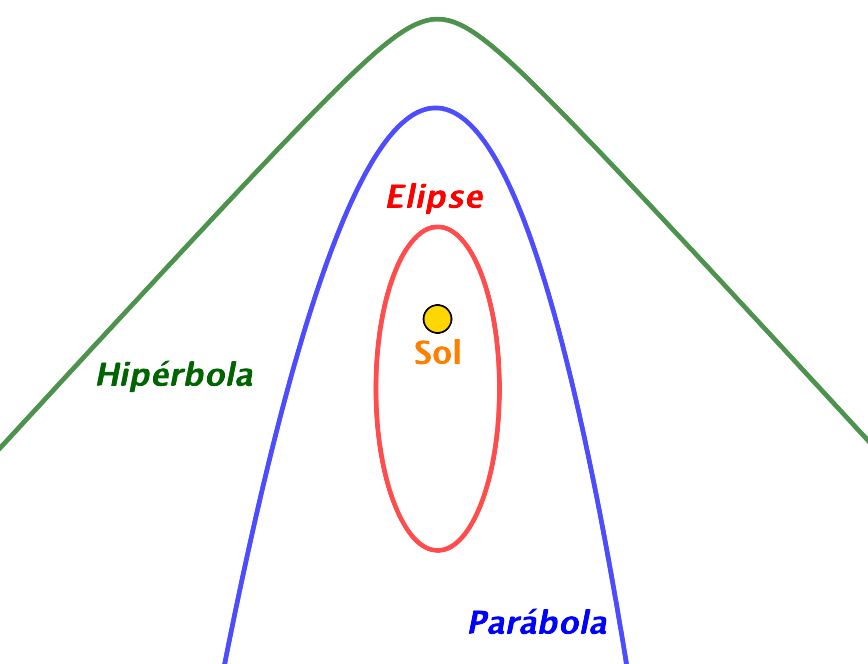
\includegraphics[width=.35\textwidth]{imagenes/imagenes15/T15IM02.png}
\end{figure}
\end{multicols}
\end{miparrafodestacado}

------ Pero, ?`por qué Keppler y Newton observaron solo órbitas elípticas?

Recordemos que teníamos la ecuación (\ref{r-theta-2}):  

$$\left( \dv{r}{\theta} \right)^2 = r^2 \ \left[ \dfrac{2G(M+m)\mu^2\ r}{L^2_{CM}}+ \dfrac{G(M+m) \mu^2 k \ r}{L^2_{CM}} - 1   \right]$$

que hemos comparado con la ecuación (\ref{elpise-polares}):

$$\left( \dv{r}{\theta} \right)^2 = r^2  \left[ \dfrac{2 \ r}{l}+\dfrac{(\epsilon^2-1) \ r^2}{l^2} - 1 \right]	$$

Identificando términos semejantes, se obtiene:

$$\dfrac {\epsilon^2-1}{l}=	\dfrac{\mu^2 G (M+m) K}{L^2_{CM}}; \qquad \qquad \dfrac{2r}{l}=\dfrac{2G(M+m)\mu^2}{L^2_{CN}} $$

De donde, $\quad l=\dfrac {L^2_{CM}}{\mu^2 G (M+m)} \ \text{ y } \ \boldsymbol{K= \dfrac{\epsilon^2-1}{l}}; \quad  \textcolor{gris}{\epsilon=\dfrac c a ;\quad c^2=a^2-b^2}$	

Veamos qué valores puede tomar $\boldsymbol k$ para que la órbita sea una u otra cónica.

$\epsilon =\dfrac c a < 1\ $ para la elipse $\ \to \ k=\dfrac{c^2-a^2}{la^2}=-\dfrac{b^2}{la^2}=-\dfrac{b^2}{b^2a}=-\dfrac 1 a$

Para la parábola: $\ \epsilon=1 \ \to \ k=0$

Para la hipérbola $\epsilon=\dfrac c a;\quad c^2=b^2-a^2 \quad \to \quad k=\dfrac 1 a $

Reuniendo estas conclusiones con la velocidad de la partícula, ec (\ref{v-cuadrado}):

\begin{miparrafodestacado}
\begin{table}[H]
\centering
\begin{tabular}{lll}
$\epsilon<1\quad$ & Elipse$\quad$ & $v^2=G(M+m)\left(\dfrac 2 r-\dfrac 1 a \right)$ \\ \\
$\epsilon=1$      & Parábola      & $v^2=\dfrac{2G(M+m)}{r}$                        \\ \\
$\epsilon>1$      & Hipérbola     & $v^2=G(M+m)\left(\dfrac 2 r+\dfrac 1 a \right)$
\end{tabular}
\end{table}	
\end{miparrafodestacado}

------ Pero, ?`qué significado tiene $\epsilon$ desde el punto de vista físico?

$\displaystyle l=\dfrac{L^2_{CM}}{\mu^2 G (M+m)};\quad \boldsymbol{ \epsilon^2-1=k l } = k \dfrac{L^2_{CM}}{\mu^2 G (M+m)} \ \to \ $

$$\epsilon \ = \ \sqrt{1+\dfrac{L^2_{CM}}{\mu^2 G(M+m)}}$$

\textcolor{gris}{$\epsilon=\dfrac c a >0$, siempre positiva, cociente de la longitud de dos segmentos.}

\begin{miparrafodestacado}
\begin{table}[H]
\centering
\begin{tabular}{lll}
 Elipse$\quad$ & $\epsilon=\sqrt{1-\dfrac{L^2_{CM}}{\mu^2 G (M+m} a}$ \\ \\
 Parábola      & $\epsilon=1$                        \\ \\
 Hipérbola     &  $\epsilon=\sqrt{1+\dfrac{L^2_{CM}}{\mu^2 G (M+m} a}$
\end{tabular}
\end{table}	
\end{miparrafodestacado}

--- La elipse es una órbita cerrada $\ \to \ $ sistema ligado.

--- La parábola e hipérbola no son cerrados $\ \to \ $ sistemas no ligados.

Un sistema de dos cuerpors en \emph{ligado} cuando ambos describen órbitas elípticas sobre el $CM$ (que estará en un foco de ambas elipses).

Si la órbita es parabólica, la velocidad es crítica. Ocurre cuando un sistema pasa de ligado a no ligado, adquiera la velocidad de escape (parabólica):

$$v^2 \ = \ \dfrac {2G(M+m)}{r} \to \text{velocidad de escape: }\ \subrayado{\ \boxed{ \ \boldsymbol{ v=\sqrt{\dfrac {2G(M+m)}{r}} } \ }\ }$$

Esta velocidad de escape no es constante, depende de $r$ y $m$ (\textcolor{gris}{la masa de un cohete que quema combustible varía}.)

Aproximación:  $\quad M>>m \ \to \ \boldsymbol{ v=\sqrt{\dfrac {2GM}{r}}}$


\section[Energía total gravitatoria para un sistema de dos partículas]{Energía total gravitatoria para un sistema de dos partículas\sectionmark{Energía total gravitatoria}}
\sectionmark{Energía total gravitatoria}

$\mathcal E = \mathcal E_c + \mathcal E_p = \dfrac 1 2 \mu v^2 - \dfrac{G(M+m)}{r} = \dfrac 1 2 \mu G (M+m) \left( \dfrac 2 r + k \right) -  \dfrac{G(M+m)}{r}$

$$K=\begin{cases} \ -1/a & :E \\ \ \ \ \ 0 & :P \\ \ \ 1/a & :H \end{cases} \quad \to \quad \qquad \subrayado{\ \begin{cases} \ E: & \quad \mathcal E=-\dfrac{GMm}{2a} \\ \ P: & \quad \mathcal E=0 \\ \ H: & \quad \mathcal E = +\dfrac{GMm}{2a} \end{cases} \ }$$

Esto nos permite hablar de \emph{sistemas ligados, $\mathcal E<0$} y \emph{sistemas no ligados, $\mathcal E\geq 0$}.

\begin{multicols}{2}
Supongamos que lanzamos un satélite desde la Tierra. Después de alcanzar su máxima altura $h$ debida al lanzamiento, recibe, en el punto $A$ (ver figura) un impulso final que le comunica una velocidad horizontal $v_0$.

La energía total de satélite en $A$ es:

\vspace{2mm} %********************************** 
$\quad E=\dfrac 1 2 m v_0^2 -\dfrac {GMm}{R+h}$

\vspace{2mm} %**********************************
La órbita será una elipse, parábola o hipérbola, según la energía total sea negativa, cero o positiva.
\begin{figure}[H]
	\centering
	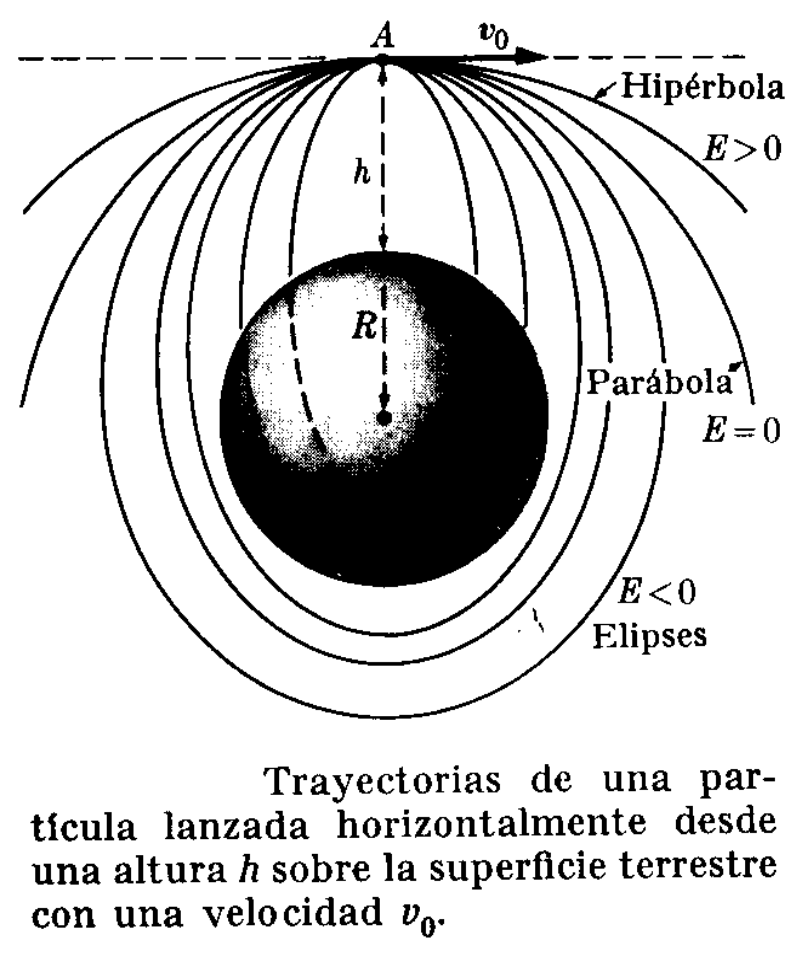
\includegraphics[width=.5\textwidth]{imagenes/imagenes15/T15IM09.png}
\end{figure}
\end{multicols}

En todos los casos, el centro de la Tierra estará en un foco de la trayectoria. Si la energía es pequeña, la órbita elíptica intersectará la Tierra y el satélite volverá a ella. Si no lo fuera, se moverá en una órbita cerrada o escapará de la Tierra, dependiendo del valor de $v_0$.

El mismo razonamiento se aplica a un satélite natural como la Luna.

\section[Energía potencial gravitatoria de una partícula de masa $m$ en las proximidades de otra de masa $M$]{Energía potencial gravitatoria de una partícula de masa $m$ en las proximidades de otra de masa $M$\sectionmark{Energía potencial gravitatoria}}
\sectionmark{Energía potencial gravitatoria}

\begin{multicols}{2}
Podemos considerar la masa $M$ concentrada en su centro.

$W_{r_1,r_2}=\mathcal E_{p}(r_2)-\mathcal E_{p}(r_1)=$

$=-G(Mm)\left( \dfrac 1 {r_2} - \dfrac 1 {r_1} \right)$

$r_1=R;\ r_2=R+h \to h<<R: $
\begin{figure}[H]
	\centering
	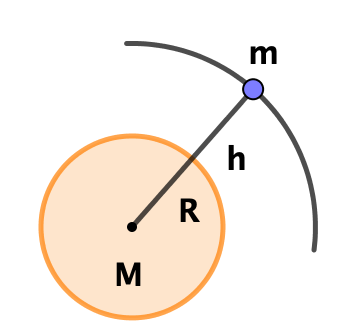
\includegraphics[width=.35\textwidth]{imagenes/imagenes15/T15IM03.png}
\end{figure}	
\end{multicols}

$W_{r_1,r_2}=-G(Mm)\left( \dfrac 1 {R+h} - \dfrac 1 {R} \right)= +G(Mm)\left( \dfrac{h}{R(R+h)} \right)$

$R>>h \ \to \ R+h \approx R \quad \to \ $

$\to \ W_{R,R+h}=\mathcal E_{p}(R+h)-\mathcal E_{p}(R)\approx \dfrac{GM}{R^2}\ m \ h=m\ g \ h$

$$\mathcal E_p(R+h)=\cancelto{0}{\mathcal E_p(R)}+mgh$$ 

por comodidad, elegimos el origen de potenciales sobre la superficie de la Tierra.
 
 
 Recordemos que teníamos la condición de que el campo fuese homogéneo, es decir, $\ \mu \left( \dfrac{\vec F_i^{(e)}}{m_i} - \dfrac{\vec F_j^{(e)}}{m_j} \right)=0$
 
\section{Órbitas y perturbaciones planetarias}
 
 La condición de homogeneidad se cumple salvo que hayan dos planetas muy cerca (Júpiter y Saturno). Las órbitas de los planetas no son perfectamente elípticas.
 
 $\displaystyle \vec  F_i^{(e)} = -G \ m_i \  \sum_{k=1}^{TCU} \  \dfrac{m_k}{r^2_{ik}} \ \vec u_{ik} ; \quad 
 \vec  F_j^{(e)} = -G \ m_j \  \sum_{k=1}^{TCU} \  \dfrac{m_k}{r^2_{jk}} \ \vec u_{ik}$
 
 Con $TCU=\text{todos los cuerpos de universo}.$
 
 Luego, $\ \displaystyle \mu \ G \left( G \ m_j \  \sum_{k=1}^{TCU} \  \dfrac{m_k}{r^2_{jk}} \ - \ G \ m_i \  \sum_{k=1}^{TCU} \  \dfrac{m_k}{r^2_{ik}} \ \vec u_{ik} \right)\ = \ 0  $
 
 Como los vectores de posición de dos cuerpos próximos son aproximadamente iguales, la igualdad anterior será 
 
  $\ \displaystyle \mu \ G \left( G \ m_j \  \sum_{k=1}^{TCU} \  \dfrac{m_k}{r^2_{jk}} \ - \ G \ m_i \  \sum_{k=1}^{TCU} \  \dfrac{m_k}{r^2_{ik}} \ \vec u_{ik} \right)\ \approx \ 0  $
  
  El hecho de que las órbitas no fuesen perfectamente elípticas determinó el descubrimiento de Neptuno.
  
\section{Problemas temas anteriores}

\begin{prob}
El diámetro del planeta Venus es $0.9777$ el de la Tierra y su densidad media es de $5\ \mathrm{g\ cm}^{-3}$. Determinar la velocidad parabólica de escape para dicho planeta, desde una altura de su superficie de $10000\ \textrm{m}$. Datos: Radio de la Tierra $6370\ \mathrm{km}$, constante de gravitación universal $G=6.674\times 10^{-1} \ \mathrm{N\ m}^2 \ \mathrm{Kg}^{-2}$.
\end{prob}

$R$, radio de venus; $h$, altura desde Venus donde calcular la velocidad de escape ($v_E$); $\rho$, densidad de Venus; $R_T$, radio de la Tierra.

Distancia desde donde calcular la velocidad de escape hasta el centro del planeta Venus: $r=R+h$

$W_{h,\infty}=\displaystyle \int_{R+h}^\infty F_{peso} \ \dd r = \int_{R+h}^\infty m\ g\ \dd r$

En la superficie del planeta, $\ g_0=\dfrac{GM}{R^2}$; a una distancia $r,\quad g=\dfrac{GM}{r^2}$, luego $\ \dfrac{g}{g_0}=\dfrac{R^2}{r^2}\ \to \ g=\dfrac{R^2}{r^2}g_0$ .

$\displaystyle W_{1,\infty} \int_{R+h}^\infty m\ g_0\ R^2 \ \dfrac{\dd r}{r^2} = m\ g_0 \ R^2 \ {\left[ -\dfrac 1 r\right]}_{R+h}^\infty=\dfrac {m\ g_0\ R^2}{R+h}$

Como $ \textcolor{gris}{\left[ \underset{R>>h}{R+h\approx R} \right]} \to \quad W_{1,\infty}= m\ g_0\ R$

Por otra parte, $W_{1,\infty}=\Delta \mathcal E_c=\dfrac 1 2 \ m \ v_E^2-0$, luego:

$\dfrac 1 2 \ \cancel{m} \ v_E^2 \ = \ \cancel{m} \ g_0\ R \quad \to \quad  \boldsymbol{v_E=\sqrt{2\ g_0\ R}= \sqrt{\dfrac{2GM}{R}}}$

$R=0.9777 R_T=6227949 \ \textrm{m}$; $\ \rho=5\ \mathrm{g\ cm}^{-3}=5 \times 10^{3}\ \mathrm{kg\ m}^{-3}$

Solo nos falta $M$, la masa de Venus: $\ M=V\ \rho = \dfrac 4 3 \pi R^3 \rho= 5.059\times 10^{24}\ \mathrm{m}^3$

Sustituyendo valores en $v_E= \sqrt{\dfrac{2GM}{R}}$, obtenemos \ $v_E\approx 10413 \ \mathrm{m\ s}^{-1}=10.4 \ \mathrm{km\ s}^{-1} = 37486  \ \mathrm{Km\ h}^{-1}$

\begin{prob}
?`Dónde pesa más un cuerpo, a $50 \mathrm{m}$  de altura	 o a $100 \mathrm{m}$ de profundidad.
\end{prob}
\begin{multicols}{2}
A $100 \ \mathrm{m}$ de profundidad, la masa $M'$ de la Tierra es:

\small{$M'=\rho \dfrac 4 3 \pi (R-100)^3=$}

\small{$ \dfrac{M}{\dfrac 4 3 \pi R^3} (100-R)^3= M \dfrac{(R-100)^3}{R^3}$}
\begin{figure}[H]
	\centering
	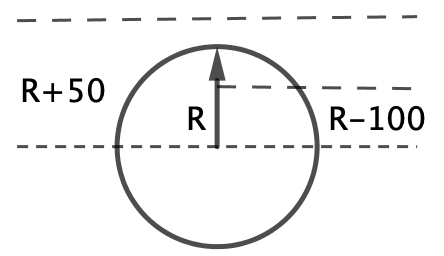
\includegraphics[width=.35\textwidth]{imagenes/imagenes15/T15IM08.png}
\end{figure}		
\end{multicols}

$F_{100\downarrow}=-\dfrac{GM'm}{(R-100)^2}=-G M \dfrac{(R-100)^3}{R^3} \dfrac{m}{(R-100)^2}= -\dfrac{GMm}{R^2} \dfrac{R-100}{R}$

Teniendo en cuenta que, en la superficie de la Tierra $F_S= -\dfrac{GMm}{R^2}$,

$F_{100\downarrow}=F_S \left( 1 - \dfrac{100}{R} \right)$

Veamos la fuerza a $50 \ \mathrm{m}$ de altura, $F_{\uparrow}$

 $F_{50\uparrow} = -\dfrac {GMm}{(R+50)^2}=  -\dfrac {GMm}{R^2 \left( 1+\dfrac{50}{R} \right)^2}=-\dfrac {GMm}{R^2} \dfrac {1} {\left( 1+\dfrac{50}{R} \right)^2} =$ 
 
 $=-\dfrac {GMm}{R^2} \dfrac {1} {1+\dfrac {100}R + \cancelto{0}{\dfrac{2500}{R^2}}}\approx -\dfrac {GMm}{(R+50)^2} \dfrac 1 {1+\dfrac{100}{R}}$

Comparando con $F_S$, $\ F_{50\uparrow}=F_S \dfrac 1 {1+\dfrac{100}{R}}$

Comparemos ambas fuerzas: 

$\dfrac{F_{50\uparrow}}{F_{100\downarrow}}=\dfrac{F_S \dfrac 1 {1+\dfrac{100}{R}}}{F_S \left( 1 - \dfrac{100}{R} \right)} = \dfrac{\dfrac R{R+100}}{\dfrac{R-100}R}=\dfrac{R^2}{R^2-10000}>1$

Luego, aunque muy ligeramente, $\ F_{50\uparrow}\ > \ F_{100\downarrow}$

\begin{prob}
Discutir la variación de la aceleración de la gravedad que tiene lugar cal desplazarse	una pequeña distancia $h$ hacia arriba o hacia abajo de la superficie de la Tierra.
\end{prob}

 ------Puntos sobre la superficie de la Tierra: $ \ r=R+h :$
 
 $E_{h\uparrow}=-\dfrac{GM}{(R+h)^2}=-\dfrac{GM}{R^2\left(1+\dfrac h R \right)^2}= \dfrac{g}{\left(1+\dfrac h R \right)^2}=g\left(1+\dfrac h R \right)^{-2}$
 
 Usando la \emph{aproximación del binomio} (ver apéndice \ref{McLaurin} -  McLaurin): 
 
 $\ x<<1 \ \to \ \boldsymbol{ (1+x)^n\approx 1+nx } \quad \Rightarrow \ \textcolor{gris}{h<<R\ \to \ \dfrac h R << 1}$ 
 
 $E_{h\uparrow}\approx g \left( 1-2\dfrac{h}{R} \right)=9.81-3.06\times 10^{-6} h \ \mathrm{m\ s}^{-2}$

------ Puntos por debajo de la superficie de la Tierra: $\ r=R-h : $

Como acabamos de ver en el problema anterior, al desplazarse una cantidad $h$ hacia el centro de la Tierra, la masa que hay por debajo es $M'=M{\left( \dfrac{R-h}R \right) }^3$

$E_{h\downarrow}=-\dfrac{GM'}{(R-h)^2}=-\dfrac{GM(R-h)^3}{R^3(R-h)^2}=-\dfrac{GM(R-h)}{R^3}=-\dfrac{GM}{R^2} \dfrac{R-h}{R}$

$E_{h\downarrow}=g\left( 1-\dfrac h R \right) =9.81-1.53\times 10^{-6}h\ \mathrm{m\ s}^{-2}$

En ambos casos la gravedad disminuye, pero lo hace más rápidamente para puntos situados sobre la superficie de la Tierra que para puntos puntos por debajo.




\begin{prob}
 Suponiéndose que pudiera escavarse un túnel a través de la Tierra de un lado a otro siguiendo un diámetro, demostrar que el movimiento de una partícula que se dejara caer en el túnel es un movimiento armónico simple (MAS). Supóngase que no existe fricción y que la Tierra tiene una densidad constante. ¿Cuánto tiempo tardará en atravesarla?
\end{prob}

$F=-\dfrac{GMn}{r^2}=-\dfrac{Gm\dfrac 4 3 \pi r^3 \rho}{r^2}=-\dfrac{4Gm\pi \rho}{3}$

$F=-Kr \to MAS;\quad K=\dfrac{4Gm\pi \rho}{3}$

$m \ddot{r}=-kr;\quad \ddot{r}=-\dfrac k m r=-\omega^2 r$, 

con $\quad \omega=\sqrt{\dfrac k m}=\dfrac{2\pi}{T} \quad \to \quad T=2\pi\sqrt{\dfrac m k}=2\pi \sqrt{\dfrac{3 \cancel{m}}{4G\pi \rho \cancel{m}}}=\sqrt{\dfrac{3 \pi}{G \rho}}$
 
$G=6.674\times 10^{-1} \ \mathrm{N\ m}^2 \ \mathrm{Kg}^{-2}; \quad \rho=5500 \ \mathrm{kg\ m}^{-3} \ \to \ T=5067\ \mathrm{s}$

Esto es una revolución completa, ir y volver. Hacer solo uno de estos recorridos supondría un tiempo $\ T/2=2833.5\ \mathrm{s} =47,2\ \mathrm{min}\sim 0.8 \ \mathrm{h}$

\vspace{10mm} %****************************************
\begin{prob}
	Dos cuerpos de masas $m$ y $2m$ se encuentran en los vértices de un triángulo equilátero de lado $a$. Encontrar el potencial y el campo gravitatorios en el punto medio entre los vértices en que están las masas así como en el tercer vértice.
\end{prob}

\begin{multicols}{2}
------ $V$ y $E$ en el punto medio entre las dos masas:

$V_m=-G\dfrac{m}{a/2}; \ V_{2m}=-G\dfrac{2m}{a/2} \ \to V=V_m+V_{2m}=-3G\dfrac{m}{a/2}$

$V=-6G\dfrac m a$

$E_m=-G\dfrac{m}{(a/2)^2}; $

$\ E_{2m}=+G\dfrac{2m}{(a/2)^2} \ to $
\begin{figure}[H]
	\centering
	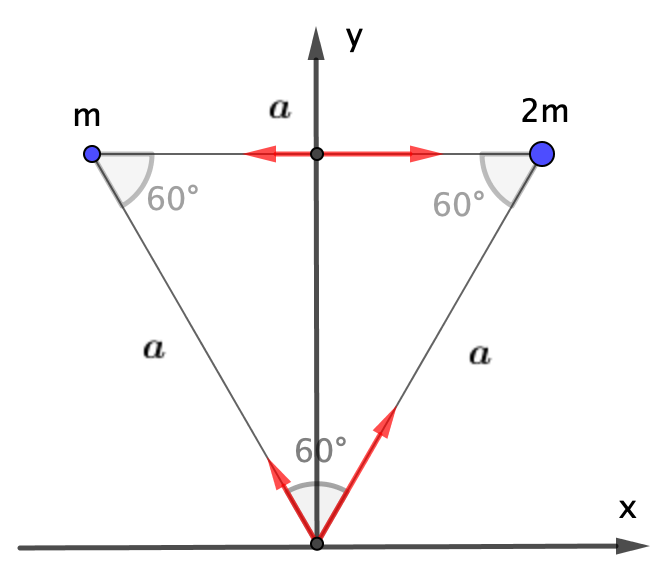
\includegraphics[width=.5\textwidth]{imagenes/imagenes15/T15IM06.png}
\end{figure}	
\end{multicols}
$E=\dfrac{Gm}{(a/2)^2}(-1+2)=+4\dfrac{Gm}{a^2}$, dirigido hacia la masa $2m$.

------ $V$ y $E$ en el tercer vértice del triángulo:

$V_m=-G\dfrac m a ;\ V_{2m}=-G \dfrac {2m} a \ \to V=V_m+V_{2m}=-3G\dfrac m a$

$E_x=\dfrac{G2m}{a^2} \cos 60^0 - \dfrac{Gm}{a^2} \cos 60^o = \dfrac 1 2 \dfrac{Gm}{a^2}$

$E_y=\dfrac{G2m}{a^2} \sin 60^0 + \dfrac{Gm}{a^2} \sin 60^o = 3 \dfrac{\sqrt{3}}2 \dfrac{Gm}{a^2}$

$\vec E=\dfrac{Gm}{a^2}\ \left( \dfrac 1 2 \vec i + \dfrac{3\sqrt{3}}2 \vec j \right)$


\vspace{15mm} %********************************************
\begin{prob}
	Las altitudes del apogeo y perigeo de un satélite terrestre son $750\ \mathrm{km}$ y $260\ \mathrm{km}$, respectivamente. Calcúlese su periodo, las velocidades máximas y mínimas del satélite así como la excentricidad de la órbita.
	
	Datos: Radio de la Tierra, $R=6370\ \mathrm{km}$; coeficiente de atracción de la Tierra, $GM=3.99\times 10^{14}\ \mathrm{UI}$ (\textcolor{gris}{UI: unidades internacionales.})
\end{prob}
 
 \newpage %****************************************************
 
 \begin{multicols}{2}
 $d_1=750\ \mathrm{km}; \ d_2=260\ \mathrm{km}$
 
 $r_1=R+d_1;\ r_2=R+d_2$
 
 
 3a. Keppler: 
 
 $\ T^4=\dfrac{4\pi^2}{GM}a^3 \to T=\dfrac{2\pi}{\sqrt{GM}}a^{3/2}$
 
 $a=r_1+r_2 =R+\dfrac{r_1+r_2}2$
 
 Datos $\to \ T=5660\ \mathrm{s}$
 	\begin{figure}[H]
	\centering
	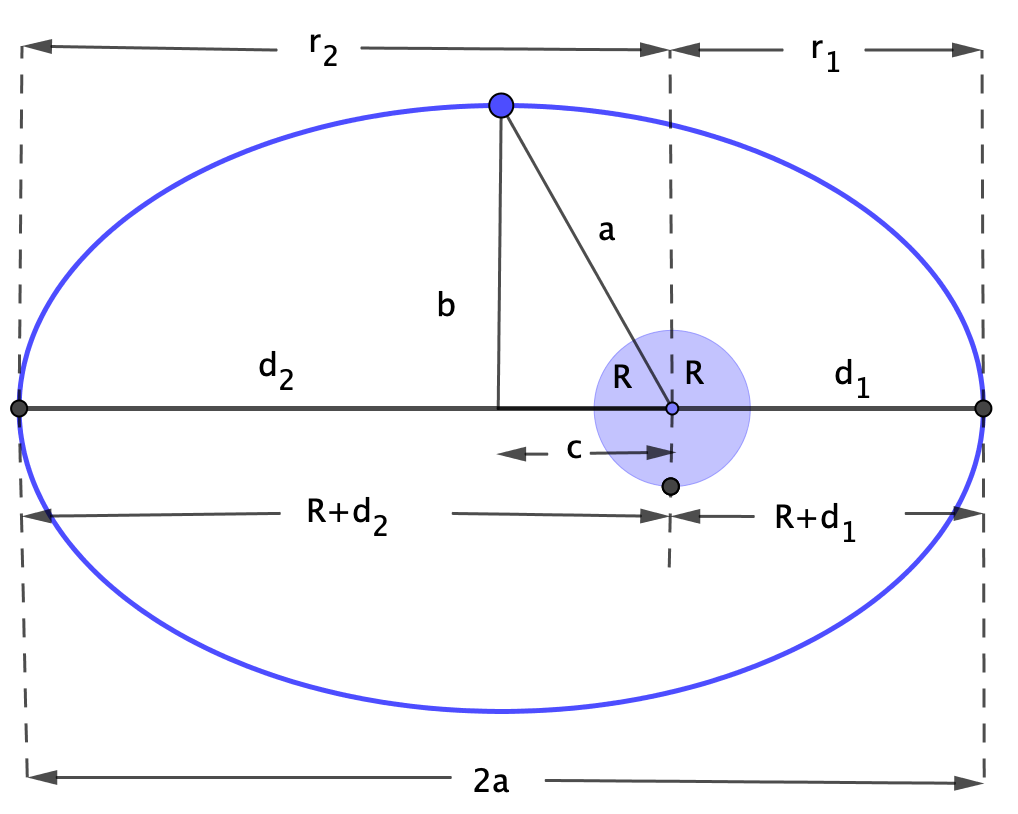
\includegraphics[width=0.5\textwidth]{imagenes/imagenes15/T15IM07.png}
\end{figure}
 \end{multicols}

La energía total se conserva (campo gravitatorio central, conservativo). En el apogeo $d_2$ (más alejado de la Tierra) la velocidad será mínima $v_m$, en el perigeo $d_1$ (punto más próximo del satélite a la Tierra), la velocidad será máxima $v_M$.

Balance energético:
$\quad E_{T}=-G\dfrac{M\cancel{m}}{2a}=\mathcal E_p+\mathcal E_c=-G\dfrac{m\cancel{m}}{r}+\dfrac 1 2 \cancel{m} v^2$ 

Para $r=r_1 \ \to \ v=v_M$

$r_1=r_2=2a; -\dfrac{GM}{2a}+\dfrac{GM}{r_1}=\dfrac 1 2 v_M^2=GM\left( \dfrac{1}{r_1}-\dfrac{1}{r_1+r_2} \right)=\dfrac{GM}{r_1+r_2} \dfrac{r_2}{r_1}$

$ v_M=\sqrt{ \dfrac{2GM}{r_1+r_2} \dfrac{r_2}{r_1} } \quad $
Para $r=r_2 \ \to \ v_m=\sqrt{ \dfrac{2GM}{r_1+r_2} \dfrac{r_1}{r_2} }$

Sustituyendo los datos, $\ v_M=7.9\ \mathrm{km\ s}^{-1};\  v_m=7.4\ \mathrm{km\ s}^{-1}$

 Excentricidad de la órbita:  $\ \epsilon = \dfrac{\sqrt{a^2-b^2}}a$
 
 $a=\dfrac{r_1+r_2}{2};\ C=a-r_1=\dfrac{r_1+r_2}{2}-r_1=\dfrac{r_2-r_1}{2}$
 
 $b^2=a^2-c^2=\dfrac{(r_1+r_2)^2}{4}-\dfrac{(r_2-r_1)^2}{4}=\cdots=r_1r_2$
 
 $\epsilon=\dfrac{\sqrt{\dfrac{(r_1+r_2)^2}{4}-r_1r_2}}{\dfrac{r_1+r_2}{2}}=\cdots=\dfrac{r_2-r_1}{r_2+r_1}$
 
 $\epsilon= \dfrac{R+d_2-(R+d_1)}{2R+d_2+d_1}=\dfrac{d_2-d_1}{2r+d_2+d_1}$
 
 Sustituyendo valores, obtenemos $\ \epsilon=0.035$

\begin{prob}
Determinar la velocidad de un cuerpo, que se suelta desde una distancia $r$ del centro de la Tierra, al llegar a la superficie de ésta.	
\end{prob}
Como $v_0=0, \quad E_0=-\dfrac{GMm}{r}$. 

Al llegar a la superficie de la Tierra, distancia al centro $R$, lo hace con velocidad $v$:
$\quad E_f=\dfrac 1 2 m v^2-\dfrac{GMm}{R}$

Si suponemos que no hay fricción con la atmósfera, la energía se conserva:

$E_f=E_0 \ \to \quad \dfrac 1 2 m v_2-\dfrac{GMm}{R}=-\dfrac{GMm}{r} \ \to \quad v^2=2GM\left( \dfrac 1 R - \dfrac 1 r \right)$

Recordando que $\dfrac{GM}{R^2}=g$, tenemos que: $\ v^2=2gR^2\left( \dfrac 1 R - \dfrac 1 r \right)$

Esta expresión también puede usarse para encontrar la distancia $r$ que alcanza un cuerpo lanzado verticalmente con velocidad $v$ desde la superficie de la Tierra.

Si el cuerpo se deja caer a gran distancia, $r>>R$, 

$\ v^2=2gR^2\left( \dfrac 1 R - \cancelto{0}{\dfrac 1 r} \right)=2gR\ \to v=\sqrt{2gR}=\sqrt{\dfrac{2GM}{R}}$,

expresión de que coincide con la velocidad de escape de un cuerpo desde la superficie de la Tierra.

La expresión anterior da, aproximadamente, la velocidad con que un meteorito choca contra la superficie de la Tierra.

\vspace{15mm} %******************************************
\begin{prob}
Determinar la altura $h$	 y la velocidad en su órbita $v$ de un satélite artificial para que sea geoestacionario, es decir, permanezca en un posición fija sobre la Tierra.
\end{prob}

\begin{figure}[H]
	\centering
	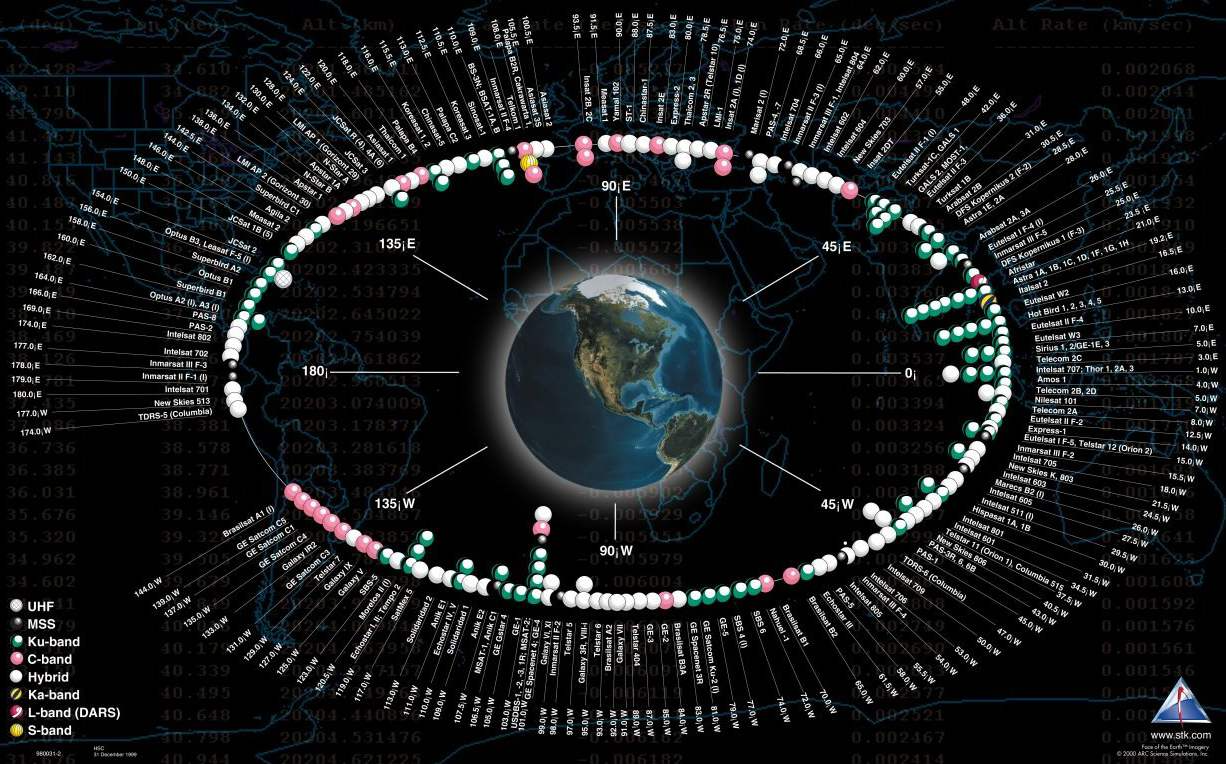
\includegraphics[width=1\textwidth]{imagenes/imagenes15/T15IM10.png}
	\caption*{Satélites en órbita geoestacionaria a lo largo del Cinturón de Clarke. Imagen de ``raiden.tk''  }
\end{figure}

Un satélite de masa $m$ que érbita a una altura $h$ sobre la superficie terrestre tiene una velocidad orbital dada por: 
$\ v=\sqrt{\dfrac{GM}{R+h}}$

\textcolor{gris}{$F_C=F_G \ \to \ m \dfrac {v^2}{R+h}=\dfrac{GMm}{(R+h)^2}$}

Para que el satélite sea geoestacionario ha de estar en una órbita paralela al ecuador terrestre y tener un periodo orbital igual al de rotación de la Tierra. Por la tercera de Keppler:

$T^2=\dfrac{4\pi^2}{GM} r^3 \ \to \ r=\left(\dfrac{GMT^2}{4\pi^2} \right)^{1/3}$

Con $\ T=24\ \mathrm{h}=86400\ \mathrm{s} \to r=4.22\times 10^{7}\ \mathrm{m};\ v=3.07\times 10^{3}\ \mathrm{m\ s}^{-1}$  

Como $r=R+h; \ R=6.37 \ \mathrm{km} \to$ el satélite estará en órbita sobre el ecuador a $h=r-R=3.58\times 10^7 \mathrm{m}=35.8 \mathrm{km}$ con una velocidad orbital de $v=3.07\times 10^{3}\ \mathrm{m\ s}^{-1}=11052 \mathrm{km\ h}^{-1}$

\begin{prob}
Una barra homogénea de masa $M$ y longitud $L$ está centrada en el origen y apoyada longitudinalmente a lo largo del eje $X$. Determinar el campo gravitatorio en un punto del eje $X$ tal que $x>L/2$. 	
\end{prob}

\begin{figure}[H]
	\centering
	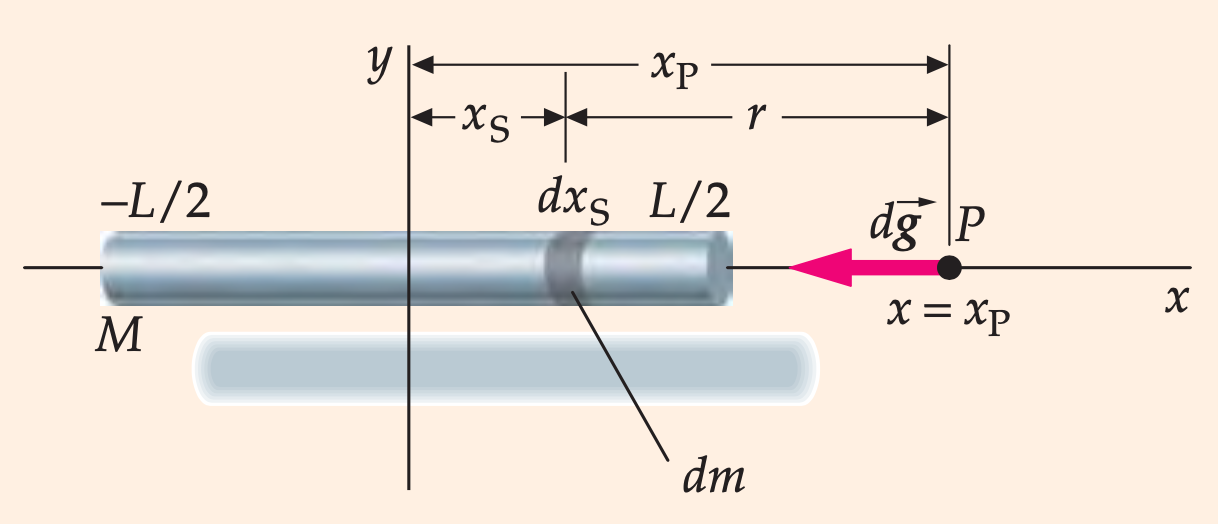
\includegraphics[width=1\textwidth]{imagenes/imagenes15/T15IM11.png}
\end{figure}

Consideramos un elemento de la barra de masa $\dd m$ situado a una distancia $x_s$ del origen y de espesor $\dd x$ y consideramos un punto $P$ en $x=x_s>L/2$.

$\dd m = \lambda \dd x$, con $\lambda=M/L$ la densidad lineal de masa:$\ \dd m =\dfrac M L \ \dd x$

El campo gravitatorio que en $P$ crea $\dd m$ es: $\ \dd E_x=-\dfrac{G\dd m}{r^2}$, con $r=x_0-x_s$

$\dd E_x=-\dfrac{GM/L\ \dd x}{(x-x_0)^2}\ $ e integraremos desde $-L/2$ hasta $+L/2$:

$E_x=-\displaystyle \int_{-L/2}^{L/2} \dfrac{GM/L\ \dd x}{(x-x_0)^2} = -(-1)\dfrac{GM}{L} \int_{-L/2}^{L/2} \dfrac{(-1) \dd x}{(x-x_0)^2}= $

$\displaystyle =- \dfrac{GM}{L} \left[ \dfrac {-1} {x_0-x}  \right]_{-L/2}^{L/2} = \dfrac{GM}{L} \left[ \dfrac 1 {x_0-x}  \right]_{-L/2}^{L/2}=$

$\displaystyle = \dfrac{GM}{L} \left[ \dfrac{1}{x_0-L/2}-\dfrac{1}{x_0+L/2} \right] = -\dfrac{GM}{x_0^2-\left(\dfrac L 2 \right)^2}$

Donde $x_0$ es un punto arbitrario del eje $X$, pero con $x_0>L/2$.

\textbf{Análisis de casos extremos: } Para $x_0>>L/2 \ \to \ E_x=-\dfrac{GM}{x_0^2}\ $ Expresión que coincide con el campo creado por una masa puntual $M$ situada en el origen de coordenadas.

\begin{prob}
Una esfera sólida de radior $R$ tiene su masa $M$ distribuida no uniformemente sino que su densidad $\rho$ es proporcional a la distancia al centro de la esfera, es decir, $\rho=Kr$, con $r\leq R$ y $K=cte$. Determinar la constante $K$ y el campo para $r\geq R$ y para $r=R/2$.
\end{prob}

\begin{figure}[H]
	\centering
	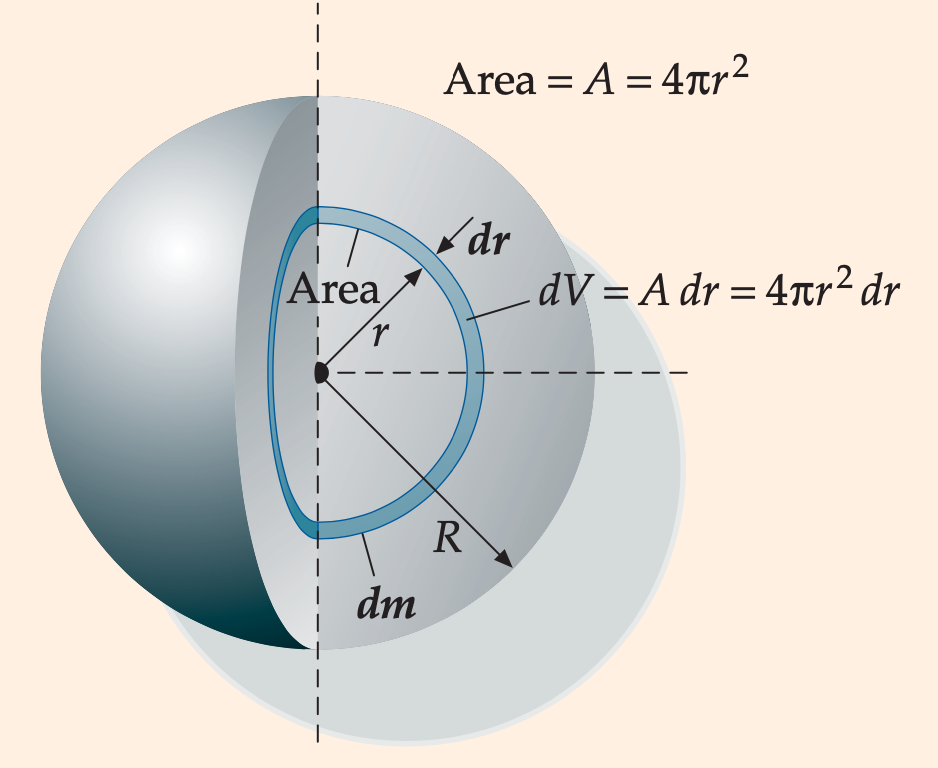
\includegraphics[width=1\textwidth]{imagenes/imagenes15/T15IM12.png}
\end{figure}

Tomamos una corteza esférica a distancia $r$ del centro, de masa $\dd m$ y espesor $\dd r$. Se tiene que:

$\displaystyle \dd m=\rho \dd V= \rho 4\pi r^2 \dd r \to M=\int \dd m =\int \rho \dd V$

$\displaystyle M=\int_0^R Kr \dd V = \int_0^R k r 4\pi r^2 \dd r= 4\pi K \int_0^R r^3 \dd r= K\pi R^4$

Por lo que $K=\dfrac{M}{\pi R^4}$

El campo gravitatorio, para $r\geq R$ es el mismo que si la masa total $M$ estuviese concentrada en el centro de la esfera:
$\ \vec E(r\geq R)=-\dfrac{GM}{r^2}\ \vec u_r$

En un punto en que $r=R/2$, el campo es el mismo que el que determinaría una esfera de masa $M'$, de radio $R/2$; la masa entre $R/2$ y $R$ no produce campo. A su vez, el campo de la esfera de masa $M'$ y radio $R/2$ es el mismo que el de una masa puntual $M'$ centrada en el centro de la esfera.

Calculemos la masa $M'$ de una esfera no homogénea de radio $R/2$:

$M'=\displaystyle \int \rho \dd V=\int_0^{R/2}\rho \dd V = \cdots = 4\pi K  \left[ r^4 \right]_0^{R/2}= K\pi \dfrac {R^2}{16} =\dfrac{M}{16}$

Así pues, $\ \vec E(r=R/2)= -\dfrac{GM'}{(R/2)^2}\ \vec u_r=-\dfrac{4GM}{16R^4} \ \vec u_r =-\dfrac{GM}{4R^2}\ \vec u_r$




 
\newpage %*********************************************
\begin{myblock}{Órbitas planetarias}
Dentro de un sistema planetario, los planetas, planetas enanos, asteroides, cometas y la basura espacial orbitan alrededor de la estrella central, el Sol en el caso del sistema solar, en trayectorias elípticas, estando el Sol en uno de los focos. Un cometa lo hace en una órbita parabólica o hiperbólica alrededor de una estrella central y no tiene un lazo gravitatorio con la estrella por tanto no se considera parte del sistema planetario de la estrella. No se han observado en el sistema solar cometas con órbitas claramente hiperbólicas. Los cuerpos que tienen un lazo gravitacional con uno de los planetas del sistema planetario, ya sean naturales o artificiales, realizan órbitas elípticas alrededor del planeta.

\vspace{2mm} Debido a las perturbaciones gravitatorias mutuas, las excentricidades de las órbitas de los planetas varían a lo largo del tiempo. Mercurio, el planeta más pequeño del sistema solar, tiene la órbita más excéntrica. El siguiente es Marte, mientras que los planetas con menor excentricidad son Venus y Neptuno.

\vspace{2mm} Cuando dos objetos orbitan sobre sí, el periastro es el punto en el que los dos objetos se encuentran más próximos el uno al otro y el apoastro es el punto donde se encuentran más lejos.

\vspace{2mm} En una órbita elíptica, el centro de masas de un sistema entre orbitador y orbitado se sitúa en uno de los focos de ambas órbitas, sin nada en el otro foco. Cuando un planeta se acerca a su periastro, el planeta incrementa su velocidad. De igual manera, cuando se acerca a su apoastro, disminuye su velocidad.	

\vspace{2mm} El descubrimiento de Neptuno no fue `accidental’ sino que obedeció a predicciones realizadas por cálculos matemáticos. En efecto, tras el descubrimiento de Urano, los astrónomos se aplicaron a determinar los parámetros de su órbita elíptica.

\begin{figure}[H]
	\centering
	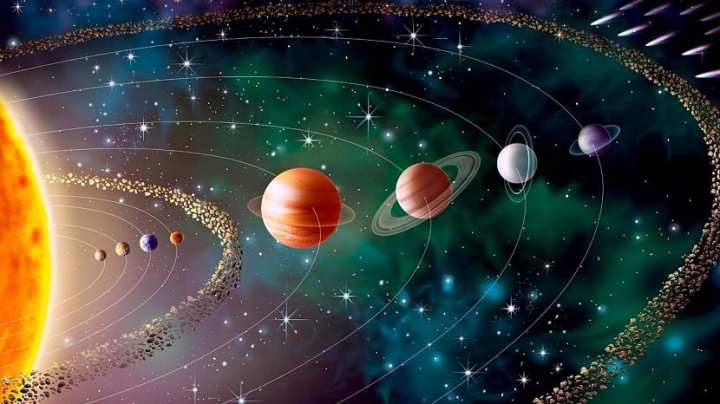
\includegraphics[width=1\textwidth]{imagenes/imagenes15/T15IM04.png}
\end{figure}

Sin embargo, según se obtenían más datos, más claro aparecía que el movimiento real del planeta se desviaba considerablemente de la órbita predicha por la teoría de la gravedad de Newton. Dado que esta teoría se encontraba firmemente establecida, pronto se generalizó la idea de que \textbf{las anomalías de Urano sólo podían deberse a las perturbaciones ejercidas por otro planeta desconocido} más lejano.

\vspace{2mm} Le Verrier en París y Adams en Cambridge realizaron los cálculos de la posición del nuevo planeta. El astrónomo alemán Johann Galle lo observó desde el observatorio de Berlín, muy próximo a la posición predicha, el 23 de septiembre de 1846.


\end{myblock}



